\chapter{Cơ sở lý thuyết}
\label{chap2}

Hệ thống khuyến nghị là 1 công nghệ hỗ trợ đắc lực cho con người, 
giúp phân tích lượng dữ liệu khổng lồ được cung cấp bởi người dùng. 
Hệ thống dự đoán điểm của các sản phẩm, tạo 1 danh sách sắp xếp thứ các 
sản phẩm này cho mỗi người dùng, và giới thiệu tới người dùng những sản 
phẩm mà họ có thể thích. Nội dung trong phần này trình bày tổng quan về 
hệ khuyến nghị, các mô hình thuật toán cùng với các kỹ thuật thuật khai 
phá dữ liệu trong hệ khuyến nghị hiện có.
\begin{figure}[htbp]
    \centering
    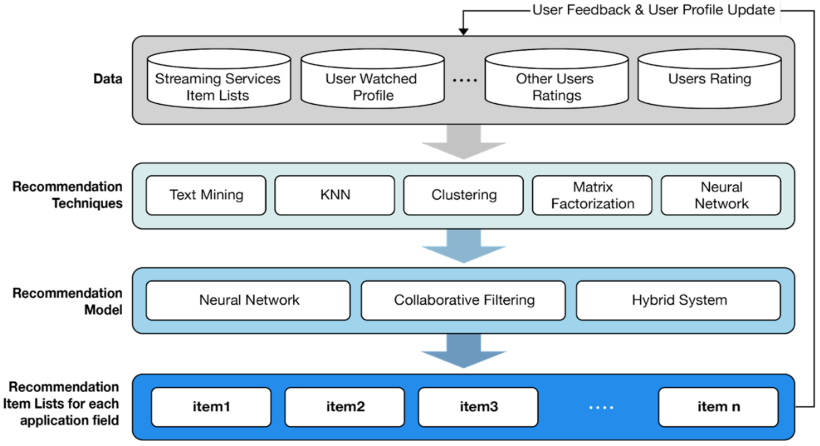
\includegraphics[width=1\textwidth]{imgs/chapter_2/tong-quan-htkn.png}
    \caption{Tổng quan hệ thống khuyến nghị}
    \label{tqhtkn}
\end{figure}
Hình \ref{tqhtkn} là tổng quan 
luồng hoạt động của 1 hệ khuyến nghị, gồm có các bước xử lý: (1) thu 
thập dữ liệu, (2) khai phá dữ liệu, (3) mô hình hóa dữ liệu, (4) và 
đưa ra gợi ý. Dữ liệu sử dụng trong hệ khuyến nghị có thể là các đánh 
giá, bình luận về sản phẩm, danh sách sản phẩm mà người dùng theo dõi, 
v.v. Các kỹ thuật khai phá dữ liệu truyền thống, có thể kể đến như: 
phân cụm, khai phá dữ liệu văn bản, KNN hay là học sâu, sử dụng mạng 
nơ-ron. Tiếp đó, các mô hình khuyến nghị sử dụng các đặc trưng đã 
được trích chọn để có thể mô hình hóa dữ liệu, từ đó đưa ra các khuyến 
nghị phù hợp tới người dùng.

Nội dung trong chương này tập trung giới thiệu và phân loại một cách tổng 
quát về các mô hình khuyến nghị hiện nay, có thể áp dụng vào bất kỳ 1 hệ thống khuyến
nghị nào.

\section{Phân loại mô hình khuyến nghị}
Các mô hình khuyến nghị có thể được chia thành 3 nhóm chính \cite{goyani2020review}:
\begin{itemize}
    \item \textbf{Lọc dựa trên nội dung}: Trong cách tiếp cận này, hệ thống sẽ thu thập các dữ
    liệu rõ ràng (điểm đánh giá sản phẩm) hoặc dữ liệu ngầm (bấm vào một đường
    dẫn) và tạo ra hồ sơ người dùng. Hệ thống sẽ thực hiện tư vấn những sản phẩm
    dựa trên những sản phẩm và hành vi liên quan tới hồ sơ người dùng. Do sở thích 
    của người dùng thường được chia thành vài nhóm cơ bản, việc chỉ sử dụng hồ sơ
    của 1 người dùng khiến hệ thống không tận dụng được thông tin từ những người
    dùng khác, từ đó hạn chế sự linh hoạt của hệ tư vấn.

    \item \textbf{Lọc cộng tác}: Không giống với lọc dựa trên nội dung, lọc cộng tác tìm kiếm
    những người dùng có sở thích tương tự nhau. Từ giả định những người dùng A
    có sở thích giống với người dùng B, hệ thống sẽ tiến hành tư vấn cho người dùng
    B những sản phẩm phù hợp người dùng A. Lọc cộng tác có 2 hướng tiếp cận: dựa
    trên bộ nhớ và dựa trên mô hình. Hướng tiếp cận dựa trên bộ nhớ tính toán độ
    tương tự giữa các người dùng từ đó thực hiện tư vấn. Nhược điểm của hướng tiếp
    cận này là sự tốn kém tài nguyên khi số lượng người dùng và sản phẩm tăng lên.
    Hướng tiếp cận dựa trên mô hình sử dụng các mô hình đã được huấn luyện thông
    qua các thuật toán học máy hoặc khai phá dữ liệu để thực hiện tư vấn.

    \item \textbf{Hệ tư vấn lai} Lọc dựa trên nội dung và lọc cộng tác đều có ưu điểm và nhược
    điểm riêng. Để giải quyết vấn đề này, hệ tư vấn lai được sinh ra, là sự kết hợp
    của 2 kỹ thuật trên.
\end{itemize}

Trong phần tiếp theo, đồ án sẽ tập trung vào việc trình bày mô hình 1 số lọc cộng
tác tiêu biểu.

\section{Lọc cộng tác}
Lọc cộng tác là một mô hình lọc thông tin, xây dựng 1 cơ sở dữ liệu sở thích người dùng 
thông qua dữ liệu tưởng tác giữa họ với sản phẩm để dự đoán các sản phẩm phù hợp với sở thích của họ, 
từ đó đưa ra các khuyến nghị về sản phẩm. Ý tưởng của mô hình lọc cộng tác là từ dữ liệu hành vi
tương tác giữa người dùng và sản phẩm, hệ thống sẽ tính toán mức độ tương đồng giữa các người dùng
hoặc giữa các sản phẩm, tạo cơ sở thực hiện khuyến nghị. Những người dùng có mức độ tương đồng cao
sẽ có xu hướng mua những sản phẩm giống nhau. Với mỗi cách tính độ tương đồng sẽ cho một mô hình lọc cộng tác 
khác nhau.

Các mô hình lọc cộng tác có thể được chia ra thông qua 2 hướng tiếp cận: lọc cộng tác dựa trên bộ nhớ và 
lọc cộng tác dựa trên mô hình. Hướng tiếp cận dựa trên bộ nhớ tính toán độ
tương tự giữa các người dùng từ đó thực hiện tư vấn. Nhược điểm của hướng tiếp
cận này là sự tốn kém tài nguyên khi số lượng người dùng và sản phẩm tăng lên. Ngoài ra, hệ 
thống cần tính toán tại thời điểm khuyến nghị, điều này sẽ ảnh hưởng tới thời gian đưa ra dự đoán.
Hướng tiếp cận dựa trên mô hình sử dụng các mô hình đã được huấn luyện thông
qua các thuật toán học máy hoặc khai phá dữ liệu để thực hiện tư vấn. Với hướng tiếp cận này, 
mô hình sẽ cần phải thực hiện huấn luyện trước, nhưng khi thực hiện khuyến nghị sẽ rất nhanh. 
Trong lọc cộng tác dựa trên bộ nhớ, ta có thể phân loại thành: 
lọc cộng tác dựa trên người dùng và lọc cộng tác dựa trên sản phẩm. Lọc cộng tác dựa trên người dùng là 
1 mô hình so sánh sự tương đồng giữa các người dùng thông qua dữ liệu tương tác của họ lên 
các sản phẩm, từ đó khuyến nghị các sản phẩm phù hợp. Lọc cộng tác dựa trên sản phẩm dự 
đoán bằng cách sử dụng độ tương đồng giữa sản phẩm và sản phẩm được chọn bởi người dùng 
thông qua 1 ma trận tương tác của người dùng và sản phẩm. Nói cách khác, lọc cộng tác dựa 
trên bộ nhớ sử dụng các kỹ thuật như: độ tương quan Pearson, độ tương quan cô-sin, KNN 
để tạo các nhóm có đặc tính giống nhau, từ đó khuyến nghị các sản phẩm tới người dùng trong 
nhóm. Do cách hoạt động dựa trên dữ liệu đánh giá, nên mô hình khó có thể hoạt động tốt 
khi không có đủ dữ liệu cần thiết. Để khắc phục vấn đề này, lọc cộng tác dựa trên mô hình 
đưa ra khuyến nghị nhờ sử dụng các thuật toán như: phân cụm, SVD hay PCA.

\subsection{Lọc cộng tác dựa trên bộ nhớ}

\begin{figure}[htbp]
    \centering
    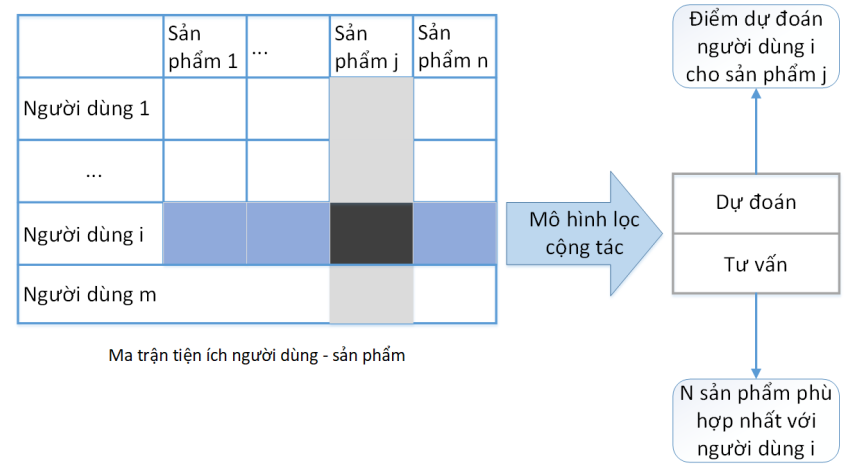
\includegraphics[width=1\textwidth]{imgs/chapter_2/loc-cong-tac.png}
    \caption{Mô hình thuật toán lọc cộng tác}
    \label{lct}
\end{figure}

\subsubsection{Lọc cộng tác dựa trên người dùng}